\graphicspath{ {imgs/} }
\documentclass[main.tex]{subfiles}
\externaldocument{02data.tex}
\externaldocument{04methods.tex}
\begin{document}
\chapter{Model}\label{chap:model}
With the building blocks defined in the previous chapter it is possible to construct a complete model for the task of lung nodule detection. This section describes in detail the used model and the learning process that was used to train it.

\section{Network Architecture}
The model is inspired by the network presented by Huang~\cite{huang2017lung}. It has $3$ 3D convolutional layers and $3$ dense layers. The full architecture can be seen in Figure~\ref{fig:net_struct} and is in the following sections explained from the input to output.

\begin{figure}
\begin{center}
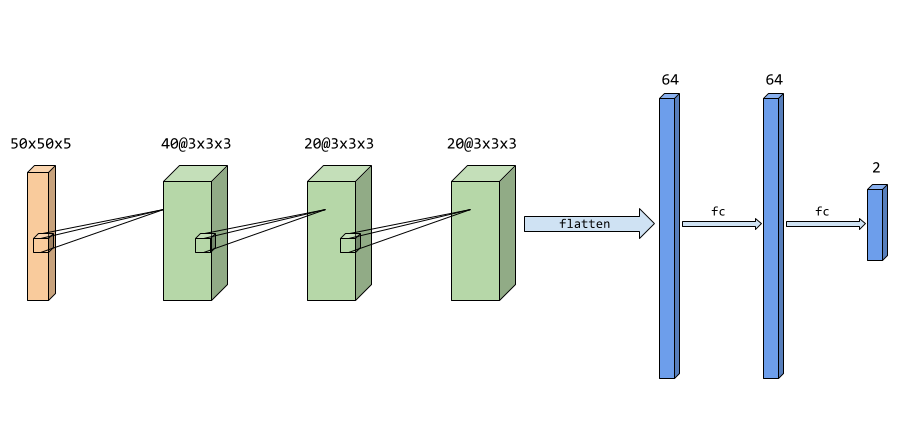
\includegraphics[scale=0.5]{net_struct.png}
\end{center}
\caption{Architecture of the neural network. Each of the convolutional layers is composed of a 3D convolution layer with the respective filter size followed by a batch normalization and a pooling layer. The pool size is $(2,2,2)$ with a stride of $(1,1,1)$. The structure of the neural network resembles the one described by Huang~\cite{huang2017lung}.}
\label{fig:net_struct}
\end{figure}

\subsection{Input} 
The input to the network are the patches that have been cut and stored from the complete lung scan as described in Chapter~\ref{chap:data} with a shape of $(50x50x5)$. The patches are randomly augmented by flipping them in x and y plane (examples can be seen in \ref{fig:input}). The augmentation is applied to make the learned classification more robust against distortions in the input and aiding in generalization. This makes sense in the specific scenario since the nodules are growing in different shapes and locations in the lung and flipping them is not producing an impossible input to the network. There is also an additional parameter that allows for scaling the input in the $x,y$ plane.

\begin{figure}
\begin{center}
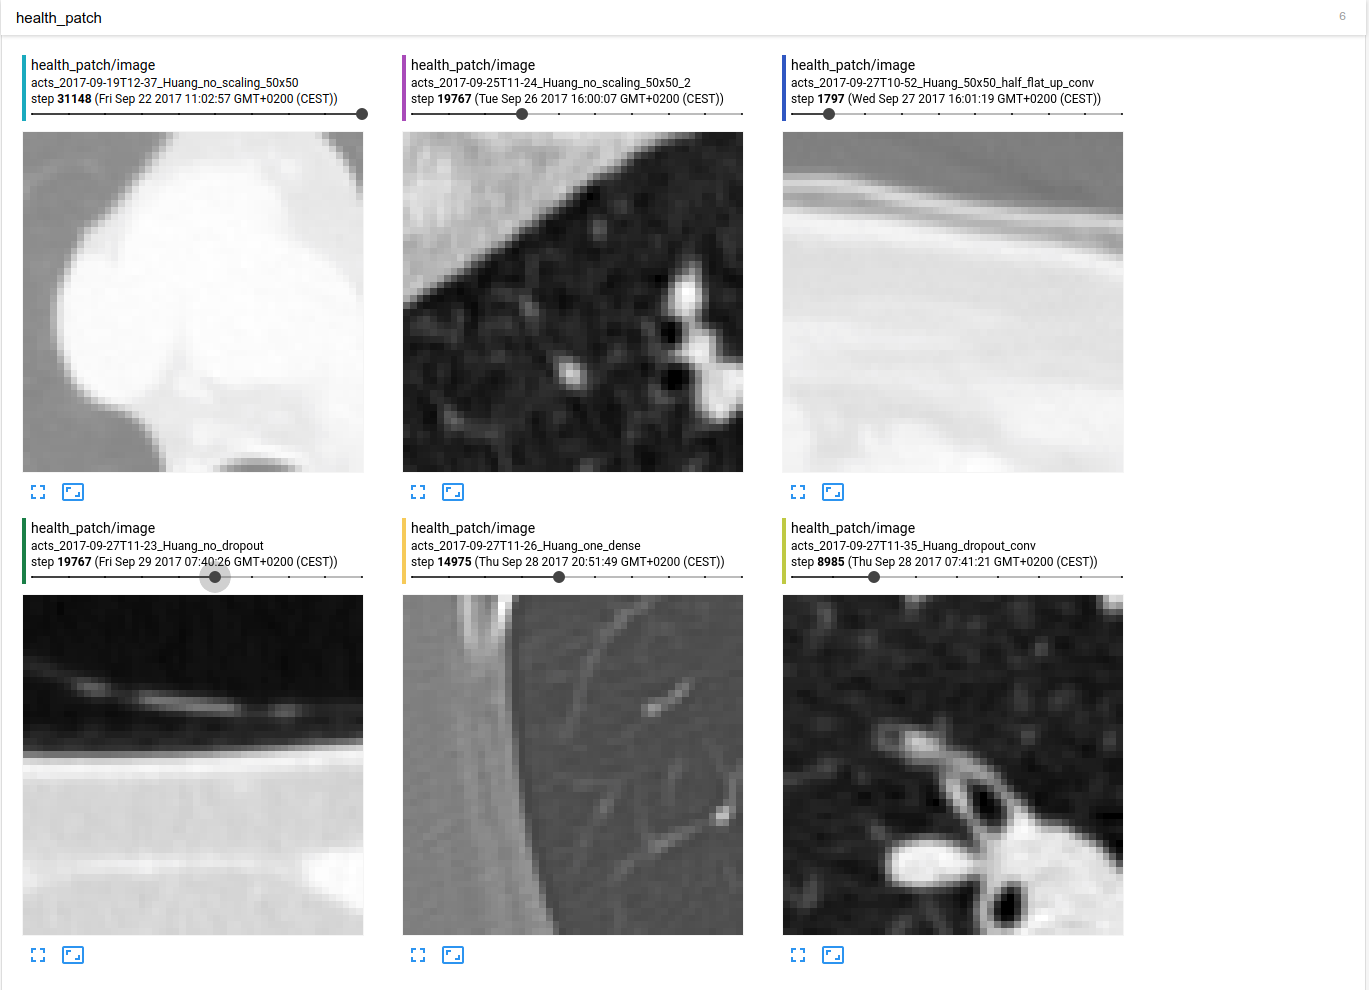
\includegraphics[scale=0.25]{patches-health.png}
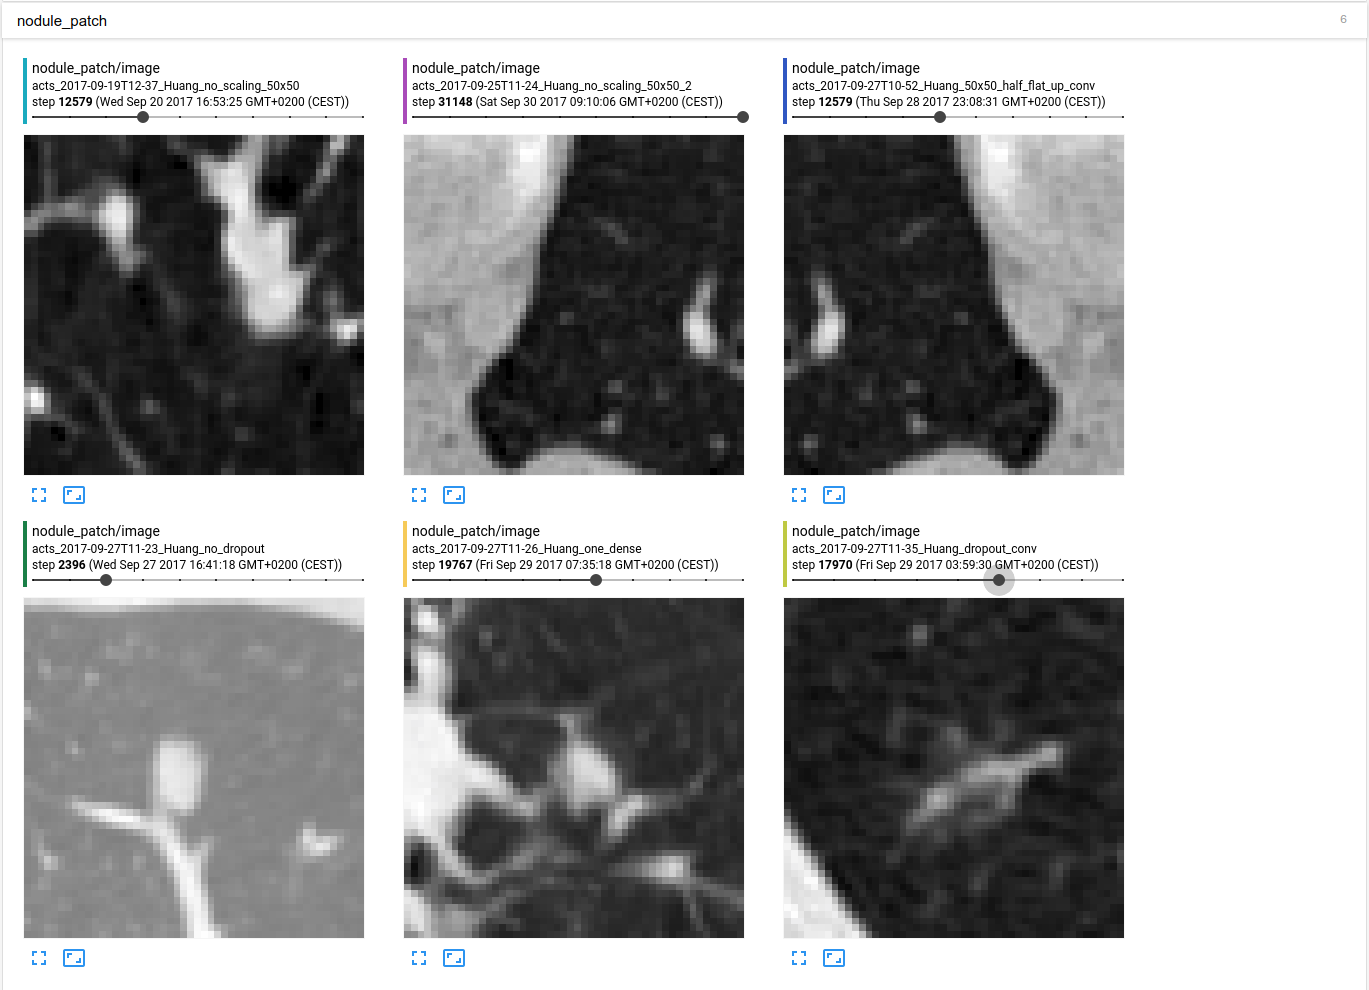
\includegraphics[scale=0.25]{patches-nodule.png}
\end{center}
\caption{Input data for the cases of healthy and nodule patches. The image is taken from Tensorboard and shows in the case of nodules the random permutation of the input data.}
\label{fig:input}
\end{figure}

\subsection{Hidden Layers}
The convolutional part has $3$ convolutional layers with $40$, $20$ and $20$ kernels each. The kernel size is $(3x3x3)$. This is in accordance with Huang et al.'s~\cite{huang2017lung} implementation. Each of them is followed by a batch normalization layer. Batch normalization is in TensorFlow implemented as described by Ioffe and Szegedy~\cite{ioffe2015batch}. The input of it is fed into a max-pooling layer with a pool size of $(2,2,2)$. The output of the last convolutional layer is flattened and fed to the dense layers. Two dense layers with $64$ neurons each and a ReLU activation function are used in this model. Their output is finally combined in two neurons, forming a 2D output of the network. 


\subsection{Output}
The output of the network is the activation of the final two neurons. The class of the input is determined by the neuron with the higher activation in an one-hot design. Given the index of the maximum, is $0$ encoding a healthy $1$ encoding a nodule patch.


\section{Training}
During training, the network is operated with batches of the input data. Regularization methods used for this network include batch normalization and dropout. Batch normalization is already described in Section~\ref{ss:convlayer}. Dropout is another regularization method which during training drops random neurons of the network - training effectively several models at once, as discovered by Srivastava et al.~\cite{srivastava2014dropout}, which should increase the overall performance of the network. During training, no improved performance could be observed when applying dropout throughout the whole network. It was rather harmful if applied to the convolutional layers. Thus, the final model uses dropout only in the fully connected layers. The loss of the network is then computed by the softmax cross-entropy between the labels in their one-hot form and the output of the two neurons at the end of the network. The Adam Optimizer is used on this loss for adapting the network parameters. For each epoch, the training is done on the complete training set with randomly permuted batches of size $10$. The training time is set to 3 full days.
                                                 


\end{document}
